\section{Check for Understanding: Vector Operations}

\begin{overview}

\textbf{Overview:} In this section, we'll apply our newly-gained knowledge about vectors.

\end{overview}

\label{act6.1.3}

\note{For Activity~\ref{act6.1.3} (\about\unit[40]{min})}{
NO Activity Sheet.

In your small group compare your responses to \FNT~\thechapter-\ref{fnt6.1.2-1} through \thechapter-\ref{fnt6.1.2-3} with other members of your small group.  Come to a consensus on an appropriate response to each \FNT{} and be able to make convincing reasons why you know for sure your response is appropriate.  Each person in your group should be prepared to do this for any of the \FNTs.  Nothing on board

Whole Class Sharing
}
\note{Note:}{
Students DO NOT put answers to the \FNTs{} up on the board.   Rather, they are to work these out among themselves at their tables.  Circulate and make sure they are getting them.  
\\[0.25in]
Then conduct a whole class discussion, going through each one as briefly as possible and calling on students to give their reasons for their answer.  Stress that they should know for sure what the appropriate response should be.
\\[0.25in]
Make sure students understand for \FNT~\ref{fnt6.2.1-1} that the magnitude of a vector is always a positive number.
}

\begin{FNTenv}
	\label{fnt6.1.2-1}Three force vectors are added together. One has a magnitude of \unit[9]{N}, the second one a magnitude of \unit[18]{N}, and the third a magnitude of \unit[15]{N}. What can we conclude about the magnitude of the net force vector?  Explain.

\begin{enumerate}[I.]
	\item It must equal \unit[42]{N}.
	
	\item It cannot be \unit[0]{N}.
	
	\item Anything from \unit[-42]{N} to \unit[+42]{N}.
	
	\item It can be anything from \unit[0]{N} to \unit[42]{N}.
	
	\item None of the above can be concluded.
\end{enumerate}
\end{FNTenv}

\vspace{-10pt}
\WCD
\vspace{3pt}

\begin{FNTenv}
	\label{fnt6.1.2-2}

Alice, Bob and Chuck are three friends standing around, talking. We know that Alice is standing \unit[9]{m} away from Bob, and that Bob is standing \unit[3]{m} away from Chuck. Let $\Delta \vec{R}_\text{AB}$ be the vector that starts at Alice and ends at Bob, and $\Delta \vec{R}_\text{BC}$ be the vector that starts at Bob and ends at Chuck.

\begin{enumerate}[(a)]
	\item Write an equation to find the displacement between Alice and Chuck.
	
	\item What is the furthest distance Chuck can be from Alice, given the information in the question? What is the closest they can be?
	
	\item Draw a picture where Chuck is neither as close as he can be or as far as he can be from Alice. Draw and label the vectors $\Delta \vec{R}_\text{AB}$ and $\Delta \vec{R}_\text{BC}$. 
\end{enumerate}
\end{FNTenv}

\vspace{-10pt}
\WCD

\begin{FNTenv}
	\label{fnt6.1.2-3}

\begin{wrapfigure}{R}{0.5\textwidth}
	\vspace{-20pt}
	\begin{center}
	\begin{tikzpicture}[thick,scale=0.65, every node/.style={transform shape},background rectangle/.style={fill=white}, show background rectangle]
		% draw a 10x7.5 grid in light gray with 5mm grid spacing
		\draw[step=.5cm,gray,very thin] (0,0) grid (10,7.5);
		% draw a darker grid in light gray with 2.5mm grid spacing
		\draw[step=2.5cm,gray,thick] (0,0) grid (10,7.5);
    
		% draw the first arrow; "Stealth" is the name of the arrowhead, and it's capitalized, so that it's scalable
		\draw[-{Stealth[scale=1.2]}, line width=1.5pt] (0.5,7) -- (2.5,5);
		% draw label A on top of the first vector
		\draw (2.5,5) node[above=12pt,align=center] {$\vec{A}$};
    
		% draw the second arrow, with descriptor B
		\draw[-{Stealth[scale=1.2]}, line width=1.5pt] (8.5,7) -- (8.5,3) node[right=3pt]{$\vec{B}$};
    
		% draw the second arrow, with descriptor C
		\draw[-{Stealth[scale=1.2]}, line width=1.5pt] (7.5,1) -- (2,1) node[above=3pt]{$\vec{C}$};

	\end{tikzpicture}
	\end{center}
	\vspace{-10pt}
\end{wrapfigure}

\noindent Using a piece of graph paper, carry out the operations listed below on the vectors shown at right. Label all vectors.

\begin{enumerate}[(a)]
	\item $\vec{A}$ + $\vec{B}$
	\item $\vec{B}$ + $\vec{A}$
	\item $\vec{A}$ - $\vec{B}$
	\item $\vec{A}$ + $\vec{B}$ + $\vec{C}$
	\item $\vec{B}$ - $\vec{A}$
	\item -$\vec{C}$
\end{enumerate}
\end{FNTenv}

\vspace{-10pt}
\WCD
\vspace{3pt}

\begin{FNTenv}
	\label{fnt6.1.2-4}

\begin{wrapfigure}{R}{0.5\textwidth}
	\vspace{-35pt}
	\begin{center}
	\begin{tikzpicture}[thick,scale=0.65, every node/.style={transform shape},background rectangle/.style={fill=white}, show background rectangle]
		% draw a 10x7.5 grid in light gray with 5mm grid spacing
		\draw[step=.5cm,gray,very thin] (0,0) grid (10,7.5);
		% draw a darker grid in light gray with 2.5mm grid spacing
		\draw[step=2.5cm,gray,thick] (0,0) grid (10,7.5);
    
		% draw the first arrow; "Stealth" is the name of the arrowhead, and it's capitalized, so that it's scalable
		\draw[-{Stealth[scale=1.2]}, line width=1.5pt] (6,5.5) -- (2,5.5);
    
		% draw the vector equation on top of the first vector
		\draw (4,5.5) node[above=6pt,align=center] {$\Sigma \vec{F} = \vec{F_1} + \vec{F_2} + \vec{F_3}$};
    
		% draw object node
		\draw (5,1) node[circle,minimum size=6pt,fill,inner sep=1pt]{} node[below=3pt]{object};
    
		% draw the second arrow, with descriptor F1
		\draw[-{Stealth[scale=1.2]}, line width=1.5pt] (5,1) -- (3,2) node[above=3pt]{$\vec{F_1}_\text{ on object}$};
    
		% draw the second arrow, with descriptor F2
		\draw[-{Stealth[scale=1.2]}, line width=1.5pt] (5,1) -- (9,5) node[above=3pt]{$\vec{F_2}_\text{ on object}$};

	\end{tikzpicture}
	\end{center}
	\vspace{-10pt}
\end{wrapfigure}

%\begin{wrapfigure}{R}{0.5\textwidth}
%	\vspace{-35pt}
 % 	\centering
%	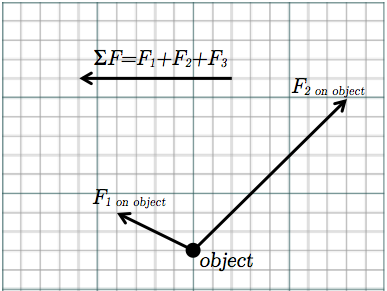
\includegraphics[height=150pt]{fnt612-4-vectors}
%	\vspace{-10pt}
%\end{wrapfigure}

\noindent Vectors $\vec{F}_\text{1 on object}$, $\vec{F}_\text{2 on object}$, and $\vec{F}_\text{3 on object}$ are all exerted on an object, adding together to form a net force vector, $\Sigma \vec{F}$, as shown in the graph to the right. However, only vectors $\vec{F}_\text{1 on object}$, $\vec{F}_\text{2 on object}$, and $\Sigma \vec{F}$ are known.\\

\noindent On a separate piece of graph paper, use the properties of vector addition to graphically determine the vector $\vec{F}_\text{3 on object}$.
\end{FNTenv}

\vspace{-10pt}
\WCD